
% Chapter 1

\chapter{Introducción general} % Main chapter title

\label{Chapter1} % For referencing the chapter elsewhere, use \ref{Chapter1} 
\label{IntroGeneral}


%----------------------------------------------------------------------------------------

% Define some commands to keep the formatting separated from the content 
\newcommand{\keyword}[1]{\textbf{#1}}
\newcommand{\tabhead}[1]{\textbf{#1}}
\newcommand{\code}[1]{\texttt{#1}}
\newcommand{\file}[1]{\texttt{\bfseries#1}}
\newcommand{\option}[1]{\texttt{\itshape#1}}
\newcommand{\grados}{$^{\circ}$}

%----------------------------------------------------------------------------------------

%\section{Introducción}

%----------------------------------------------------------------------------------------
\section{Contexto y motivación}

En las últimas décadas, la creciente demanda de energía ha generado preocupaciones significativas a nivel mundial. Este incremento en el consumo energético, impulsado por el crecimiento poblacional, la industrialización y la expansión de tecnologías dependientes de la electricidad, ha llevado a una mayor explotación de recursos naturales y un aumento de las emisiones de gases de efecto invernadero, como se observa en la Figura \ref{fig:emisionesco2}. Estos factores han contribuido al cambio climático, provocando impactos ambientales que van desde el calentamiento global hasta la pérdida de biodiversidad y eventos climáticos extremos.

\begin{figure}[ht]
	\centering
	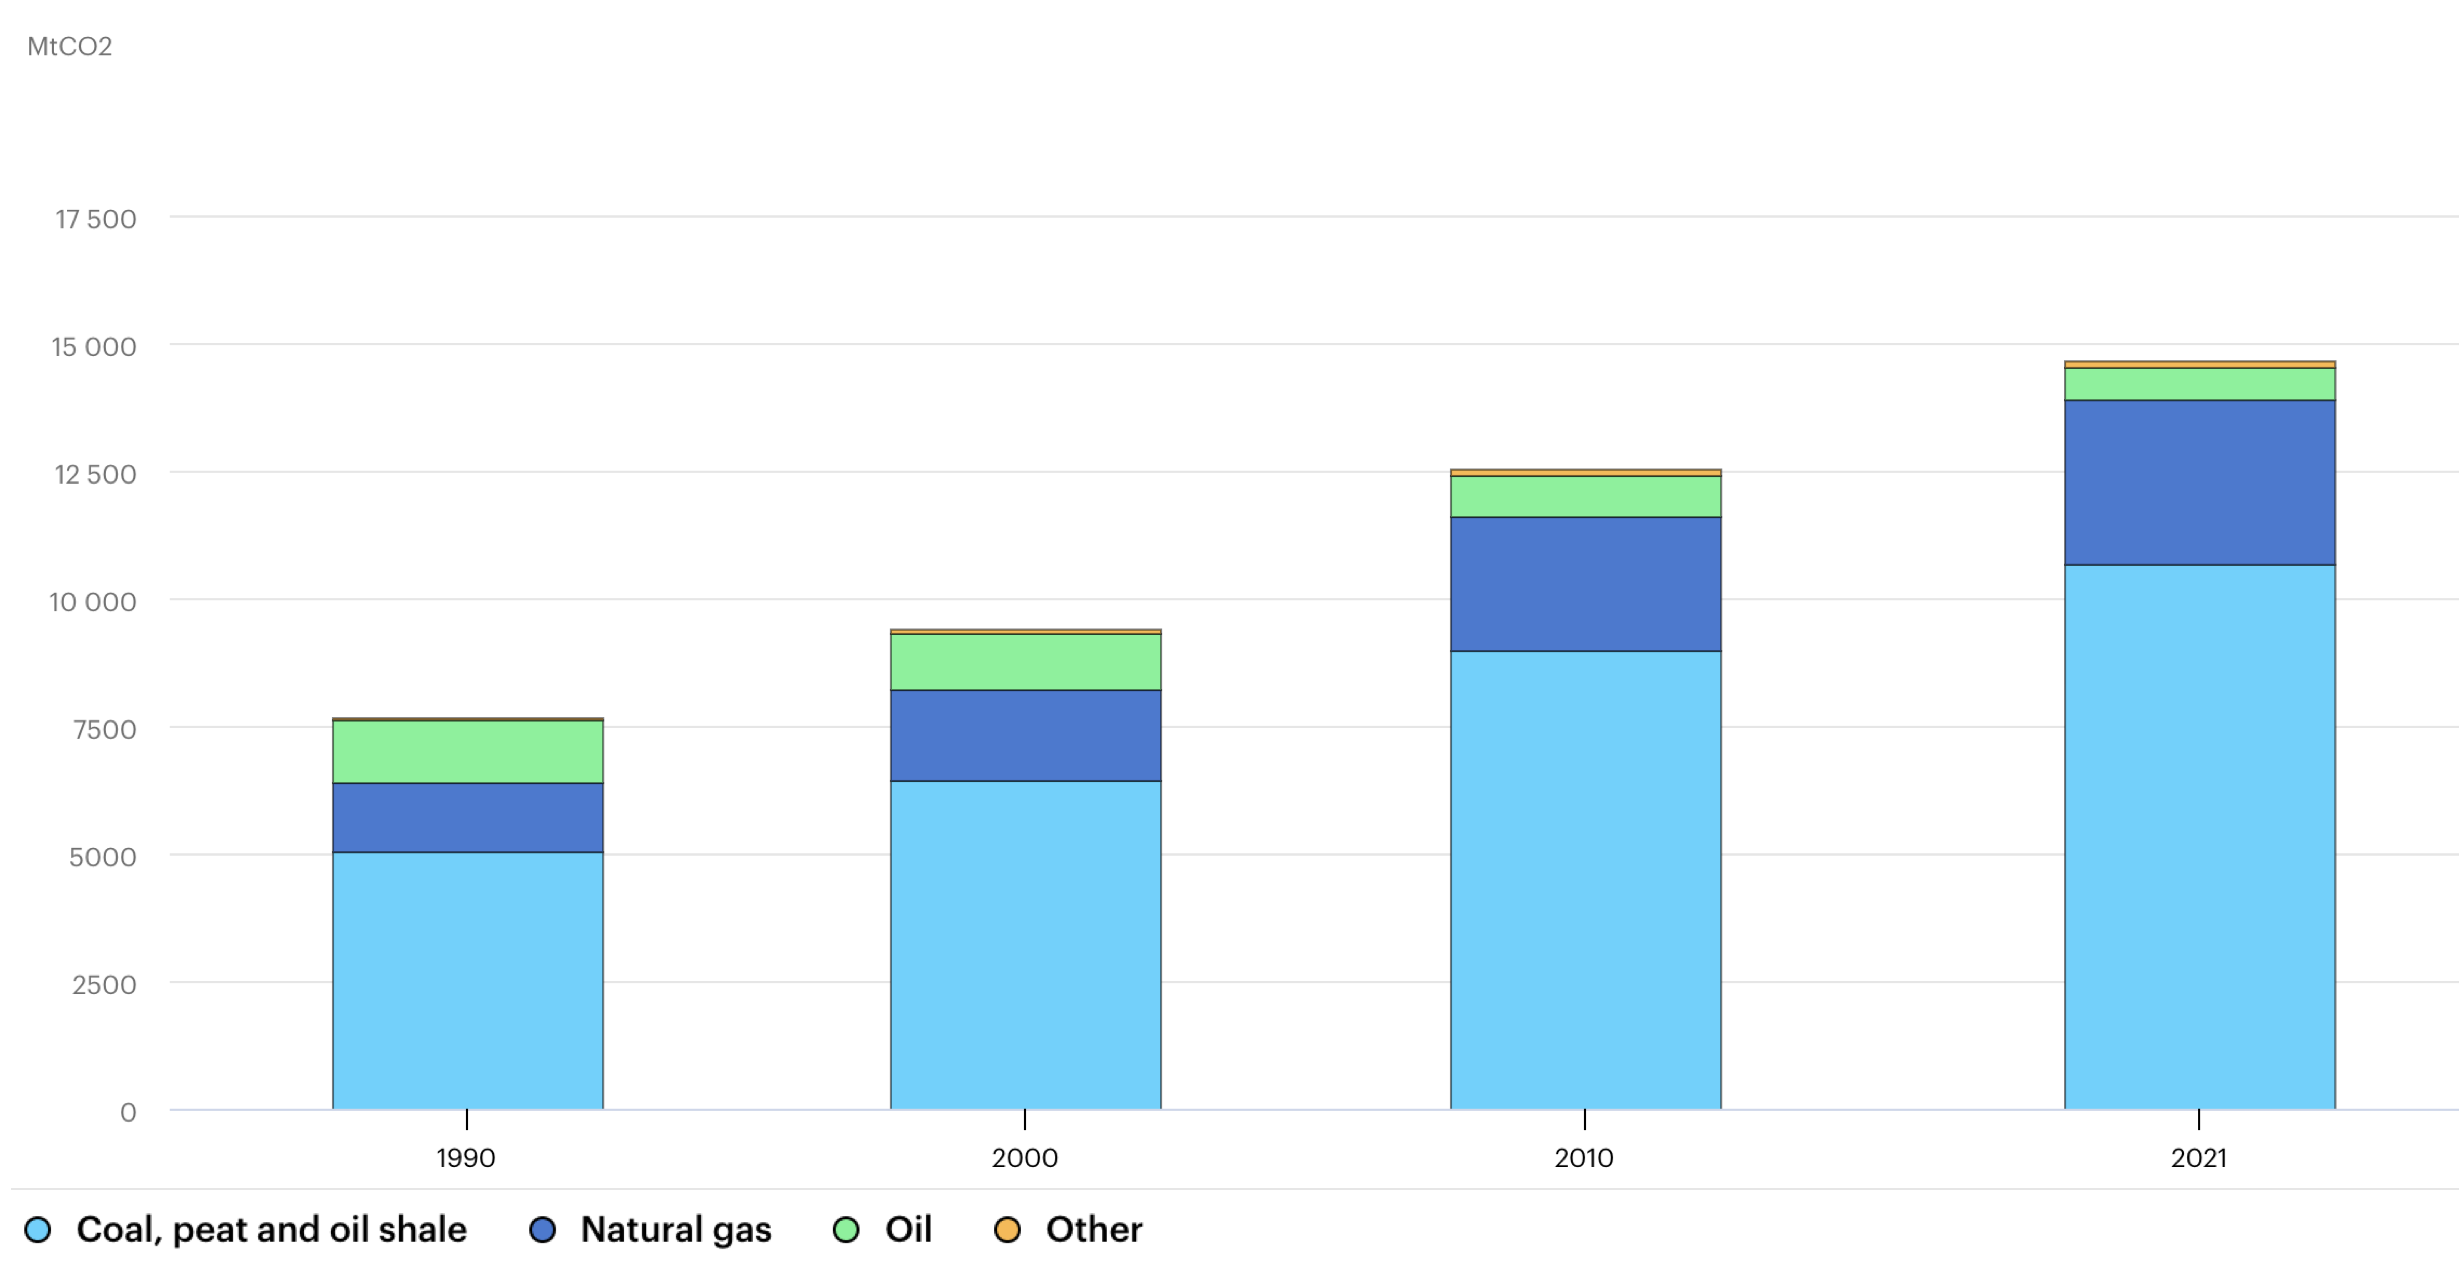
\includegraphics[width=1\textwidth]{./Figures/co2-emissions-by-electricity-generation.png}
	\caption[Emisiones de $CO_2$ por la generación de electricidad.]{Emisiones de $CO_2$ por la generación de electricidad y calor por fuente de energía, Mundo\footnotemark.}
	\label{fig:emisionesco2}
	
\end{figure}

\footnotetext{IEA (2023), Greenhouse Gas Emissions from Energy Data Explorer, IEA, Paris \url{https://www.iea.org/data-and-statistics/data-tools/greenhouse-gas-emissions-from-energy-data-explorer}}


Según un informe de la \textit{International Energy Agency} (IEA), y como se observa en la Figura \ref{fig:demandaElectricidad}, se espera que el crecimiento de la demanda global de electricidad aumente del 2,6 \% en 2023 a un promedio del 3,2 \% en 2024-2025\footnote{IEA (2023), Year-on-year change in electricity demand by region, 2019-2025, IEA, Paris \url{https://www.iea.org/data-and-statistics/charts/year-on-year-change-in-electricity-demand-by-region-2019-2025}, Licence: CC BY 4.0}. El estudio también destaca que para 2025, la demanda aumentará en 2500 TWh con respecto a los niveles de 2022, lo que significa que en los próximos tres años, el aumento anual del consumo de electricidad será aproximadamente equivalente a la suma del consumo de Reino Unido y Alemania juntos.

\begin{figure}[ht]
	\centering
	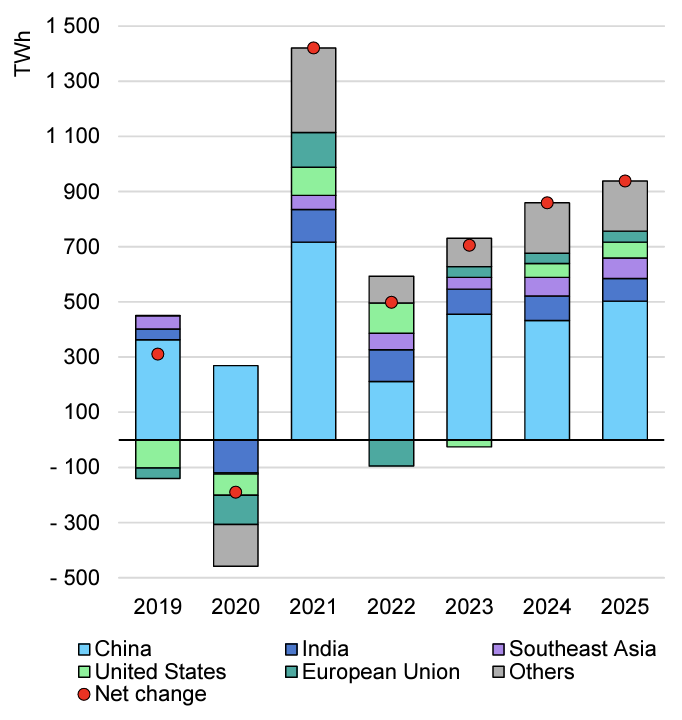
\includegraphics[width=.6\textwidth]{./Figures/year-on-year-change-in-electricity-demand-by-region-2019-2025.png}
	\caption{Cambio anual en la demanda de electricidiad por región para el período 2019-2025.}
	\label{fig:demandaElectricidad}
\end{figure}


Al mismo tiempo, el costo de la electricidad también ha experimentado un incremento significativo en los últimos años, impulsado por diversos factores como la creciente demanda, el aumento de precios de los combustibles utilizados para su generación y factores geopolíticos. Este aumento impacta directamente en el presupuesto de los hogares y en la competitividad de las industrias y la economía en general.

En este contexto, la eficiencia energética se ha convertido en una prioridad global. Gobiernos, organizaciones y consumidores buscan métodos para optimizar el uso de la energía y reducir su huella de carbono. Uno de los sectores donde esta optimización es crucial es el consumo eléctrico domiciliario. Los hogares representan una parte significativa del consumo energético total y, a menudo, carecen de herramientas eficaces para monitorear y gestionar su uso de electricidad. Esta falta de visibilidad y control sobre el consumo diario impide a los usuarios adoptar hábitos más sostenibles y económicos.

\newpage
\section{Sistema de monitoreo de consumo eléctrico}
Tener información es crucial para la toma de decisiones ya que mejora la calidad de las mismas al basarlas en hechos y datos concretos. Permite identificar oportunidades y riesgos, reduce incertidumbres, facilita la planificación estratégica y el uso eficiente de los recursos.

En el contexto anteriormente planteado, contar con información en tiempo real relacionada al consumo de energía eléctrica permitiría, por ejemplo, identificar cuáles son los electrodomésticos y hábitos que más energía consumen o tomar decisiones informadas al reemplazar o adquirir nuevos dispositivos. Disponer de información adecuada puede ayudar a los hogares a enfocar los esfuerzos de ahorro energético, disminuir sus costos asociados y contribuir a la sostenibilidad ambiental.

Es por esto que, a través de la aplicación de nuevas tecnologías y técnicas, se busca generar una herramienta innovadora, accesible y eficaz que suministre información en tiempo real sobre el consumo de electricidad de los usuarios. El objetivo primario este sistema de monitoreo de consumo eléctrico es que, a partir de los datos recolectados, los usuarios puedan tomar decisiones informadas tendientes a hacer un uso más eficiente y consciente de la energía.

\newpage
\section{Objetivos y alcance}

\subsection{Objetivos}
El principal objetivo del proyecto es el diseño e implementación de un prototipo de un producto que permita, principalmente a usuarios domiciliarios, tener información sobre su consumo de electricidad para poder tomar decisiones inteligentes que apunten a reducir el uso de energía. El objetivo subyacente es asistir a los usuarios en la reducción de costos y generar un impacto positivo en el ambiente. Este objetivo macro se desglosa en varios objetivos específicos:

\begin{itemize}
	\item Medir variables eléctricas esenciales como voltaje, corriente, potencia, frecuencia y factor de potencia.
	
	\item Asegurar que el dispositivo transmita los datos de manera confiable a un servidor en la nube para su procesamiento, almacenamiento y posterior consumo.

	\item  Proveer al usuario una interfaz intuitiva que le permita acceder a sus datos de consumo eléctrico de manera clara y comprensible.

	\item Ofrecer herramientas analíticas para identificar patrones de consumo y sugerir acciones para mejorar la eficiencia energética. 
	
	\item Fomentar el uso responsable de la energía mediante recomendaciones basadas en datos precisos.
	
	\item Educar a los usuarios sobre su consumo energético y las maneras de optimizarlo, contribuyendo a la reducción de costos y del impacto ambiental.
	
	\item Asegurar que el sistema sea escalable para adaptarse a diferentes volúmenes de datos y a un número creciente de usuarios.
	
	\item Mantener la accesibilidad y facilidad de uso del sistema, garantizando que usuarios sin conocimientos técnicos avanzados puedan beneficiarse de la herramienta.
\end{itemize}

\subsection{Alcance}

El alcance del proyecto abarca desde el diseño inicial hasta la implementación y despliegue de un sistema de monitoreo. Este sistema incluye varios componentes clave y fases de desarrollo:

\begin{itemize}
	\item Diseño y desarrollo del dispositivo de medición:
		\begin{itemize}
		\item selección de componentes de hardware y sensores adecuados para la medición de variables eléctricas.
		\item programación del dispositivo para la captura precisa de datos y su transmisión mediante conexión Wi-Fi.
		\end{itemize}
	\item Implementación de un servidor:
		\begin{itemize}
		\item configuración de una base de datos relacional para el almacenamiento seguro y eficiente de grandes volúmenes de datos.
		\item desarrollo de endpoints HTTP que permitan operaciones CRUD sobre los datos y la gestión de usuarios.
		\item implementación de un broker MQTT.
		\end{itemize}
	\item Desarrollo de plataforma web:
	\begin{itemize}
		\item creación de una interfaz de usuario intuitiva utilizando frameworks modernos.
		\item integración de funcionalidades analíticas y visualización de datos, facilitando la interpretación y el análisis del consumo eléctrico por parte de los usuarios.
	\end{itemize}
	\item Fase de pruebas y validación:
	\begin{itemize}
		\item realización de pruebas unitarias y de integración para asegurar la correcta interacción entre el dispositivo de medición, el servidor en la nube y la plataforma web.
		\item validación del sistema en un entorno real para garantizar su funcionalidad y eficacia.
	\end{itemize}
	\item Despliegue y mantenimiento:
	\begin{itemize}
		\item implementación del sistema en un entorno operativo real, disponible para usuarios domésticos.
	\end{itemize}
\end{itemize} 


\newpage

\section{Estado del arte}

